\section{Code}
\label{sec:code}

\subsection{The \sunpypkg core package}
\label{ssec:the-sunpypkg-core-package}

The \sunpypkg package is the central pillar of the \sunpyproj \citep{sunpy_community2020} and provides the fundamental tools for accessing, loading, and interacting with solar physics data in Python.
The primary components of the \sunpypkg package are summarized graphically in \autoref{fig:sunpy-core-summary} and described briefly in the following paragraphs.
For a more in-depth description of each of these components, see \citet[Section 4]{sunpy_community2020}.
The full documentation of the \sunpypkg Application Programming Interface (API) is provided in the hosted online documentation\footnote{The \sunpypkg API is fully documented here: \url{https://docs.sunpy.org}}.

\begin{figure}
    \centering
    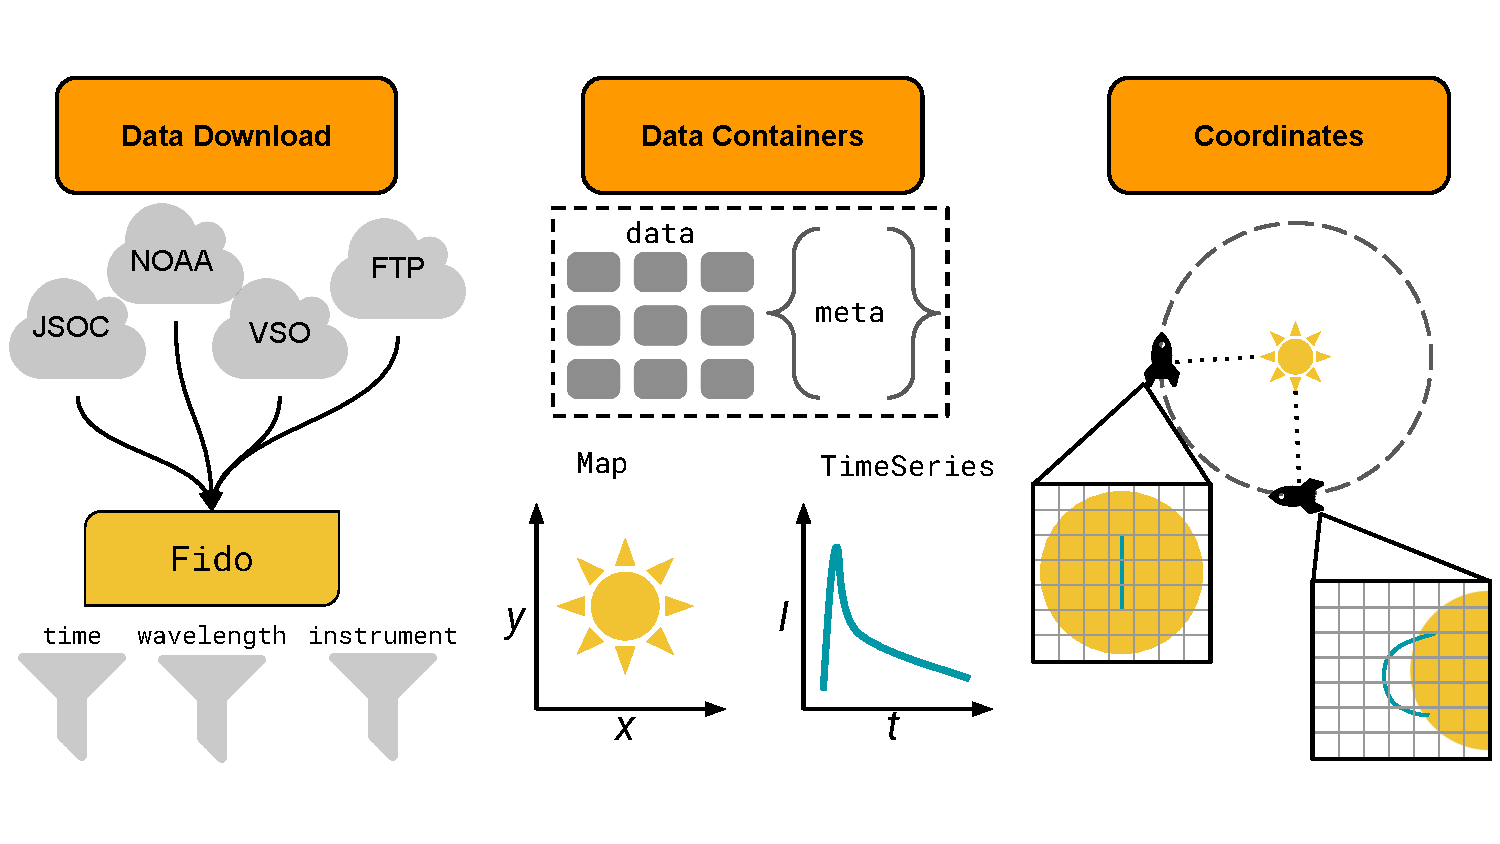
\includegraphics[width=\columnwidth]{figures/sunpy-summary-slide.pdf}
    \caption{A summary of the capabilities of the \sunpypkg core package. \sunpypkg provides search and download functionality, data containers for image and time series data, as well as commonly used coordinate frames and transformations between such frames.}
    \label{fig:sunpy-core-summary}
\end{figure}

\subsubsection{Components of the Core Package}
\label{sssec:components-of-the-core-package}

To search for and download data, \sunpypkg provides the \Fido interface for searching across a variety of data providers (e.g., the Virtual Solar Observatory (VSO)\footnote{\url{https://sdac.virtualsolar.org/cgi/search}}, or the Joint Science Operations Center (JSOC)\footnote{\url{http://jsoc.stanford.edu}}) maintained within the solar community.
\Fido internally is a collection of classes that define the search API for users including the search attributes and how a data provider interprets those attributes in order to do the final network call to any server.
A complete list of all supported data sources is provided in the documentation for using \Fido\footnote{\url{https://docs.sunpy.org/en/stable/guide/acquiring_data/fido.html}}.
Section 4.1.1 of \citep{sunpy_community2020} also provides a comprehensive discussion of the data sources that \Fido searches by default.
Additionally, \Fido can also be extended to search additional data sources that may not be included in \sunpypkg (e.g., the Solar Orbiter Archive, see \autoref{sssec:current-ecosystem}).
As illustrated in the leftmost column of \autoref{fig:sunpy-core-summary}, attributes such as time, wavelength, and instrument name, among others, can be used to filter these search results.
By providing a single interface to many disparate data sources, \sunpypkg, via \Fido, easily enables multi-instrument research workflows.

Once a user has downloaded data, the \code{TimeSeries} and \code{Map} objects can be used to load time series and two-dimensional image data, respectively.
These objects hold the data alongside the associated metadata in order to perform metadata-aware operations such as concatenation for time series or cropping for image data.
In the case of \code{Map}, a World Coordinate System \citep[WCS, e.g.,][]{greisen_representations_2002} is also constructed from the associated metadata to enable easy mapping between pixel and world coordinates via \astropypkg.

Additionally, by extending the \astropypkg coordinates framework \citep[see Section 3.3 of][for more details]{the_astropy_collaboration_astropy_2018}, \sunpypkg provides definitions of, and transformations between, common solar coordinate systems.
Coordinates expressed using these frames can be used to represent the positional information of solar features and events. \sunpypkg implements both observer-dependent (e.g., \hpc) and observer-independent (e.g., \hgs) coordinate frames \citep{thompson_coordinate_2006}.
Each \code{Map} object instance also carries with it the corresponding coordinate frame of that image and the coordinate of the observer as defined by the position of the observatory given in the associated metadata.
Whereas for \code{TimeSeries}, the metadata has a very different style as a result that there is no common format for timeseries data.
Therefore in practice there is generally little overlap between the metadata of a \code{TimeSeries} object and the metadata of a \code{Map} object.

As we will cover in \autoref{ssec:affiliated-packages}, the \sunpypkg package part of a larger ecosystem of packages that provide additional functionality for solar physics research.
So one might ask why is the \sunpypkg not simply a collection of these packages, why is there a separation of \enquote{core} vs \enquote{non-core} functionally?
The \sunpyproj defines the \enquote{core}, as the tools needed to do standard solar physics research.
This means in practice, finding and downloading data, opening the data and plotting the data.
Scientists will analyse data in so many bespoke ways that adding analysis tools without bloating \sunpypkg package is impossible.
Therefore the decision was made to ensure that the \enquote{core} enabled scientists to get to the point where they can apply their own tools on top.

\subsubsection{Testing Infrastructure}
\label{sssec:testing-infrastructure}

\sunpypkg includes thousands of unit, regression and integration tests that are run using the \code{pytest} testing framework.
This test suite is run on every pull request opened on the \sunpypkg \github repository using \github Actions to ensure that contributions to the codebase do not lead to unexpected regressions.
A full description of our testing practices can be found in our developer documentation.\footnote{A complete guide to running the tests and the associated infrastructure can be found here:\url{https://docs.sunpy.org/en/latest/dev_guide/contents/tests.html}}

\subsubsection{Release Schedule}
\label{sssec:release-schedule}

There is a new release of the core package with feature enhancements approximately every six months.
Every other release is designated a long term support (LTS) release and receives bug fixes for a year rather than for six months.
Additionally, there are bug fix releases every month.
For each release a digital object identifier (DOI) is automatically generated and a record is created on Zenodo.\footnote{The most current release on Zenodo can be found here: \url{https://doi.org/10.5281/zenodo.7314636}}
By providing regularly scheduled, versioned releases of \sunpypkg, the \sunpyproj enables reproducibility.
For example, if a researcher is attempting to reproduce a result from a paper that used \sunpypkg v2.0.2, she can create a new virtual environment and install that exact version of \sunpypkg, even if the current version is many versions ahead of v2.0.2.

This release process is completely automated through \github Actions.\footnote{The \github Actions templates used are available here: \url{https://github.com/OpenAstronomy/github-actions-workflows}}
When a release is tagged, an action is triggered that tests the package on all supported versions of Python and all supported operating systems.
If the packages build successfully, they are automatically uploaded to to Python Package Index (PyPi) and subsequently the release is updated on \code{conda-forge}.

\subsection{Affiliated Packages}
\label{ssec:affiliated-packages}

As the \sunpypkg package grew and the amount of domain- and instrument-specific code being developed in Python increased, it became increasingly challenging to store and maintain the functionality needed for all solar physics research in one package.
As such, the affiliated package system was introduced \citep{mumford_stuart_2014_3261752} so that the \sunpypkg core package could be generic enough for other packages to build on.
The goal of this system is to support and promote software packages outside the scope of the \sunpypkg core package, and to provide guidance to developers in implementing and maintaining the specific functionality provided by an affiliated package.
This fosters code-ownership while ensuring the set of affiliated packages are interoperable and follow a set of common standards (see \autoref{sssec:application-process}).
The \sunpyproj provides development support through our community development efforts and by providing a package template as a foundation.
In addition, affiliated packages are advertised at conferences and workshops where a \sunpy poster, talk, or tutorial is given.

As a result of the creation of the affiliated package ecosystem, components of the \sunpypkg core package that were tied directly to specific instruments or data analysis methods have recently been moved out into other affiliated packages.
One example of this is \aiapypkg \citep{barnes_aiapy_2020}, a package for processing data from the Atmospheric Imaging Assembly \citep[AIA,][]{lemen_atmospheric_2012} on the \textit{Solar Dynamics Observatory} \citep[SDO,][]{pesnell_solar_2012}.
Prior to version 2.1, \sunpypkg included functionality for calibrating level 1 AIA data.
In 2019, in collaboration with the \sunpyproj, the AIA instrument team began developing \aiapypkg to provide a number of AIA-specific analysis routines in Python, including the aforementioned calibration software.
\aiapypkg became an affiliated package in 2020 and the AIA-specific functionality that previously lived in \sunpypkg was deprecated and subsequently removed.
This relocation of the code allows the AIA instrument team to have full autonomy over their calibration routines and release updates to their software on a more frequent timescale than that of the \sunpypkg core package.
At the same time, \aiapypkg users and developers are able to take full advantage of the \sunpyproj ecosystem.

Outside of the current list of affiliated packages, current and future NASA and ESA missions \footnote{This includes, but is not limited to, the Interface Region Imaging Spectrometer (IRIS), several instruments on \textit{Solar Orbiter}, as well as the X-Ray Telescope (XRT) and the Extreme ultraviolet Imaging Spectrometer (EIS) onboard \textit{Hinode}}, as well as ground-based telescopes, such as the Daniel K. Inouye Solar Telescope (DKIST), have begun developing user tools for data analysis and/or pipelines for data calibration built on top of the \sunpy ecosystem.
While these packages are not yet affiliated, the \sunpyproj has assisted in coordinating development efforts between these teams in order to foster a more interoperable ecosystem.

\subsubsection{Application Process}
\label{sssec:application-process}

The affiliated package application process is completed in the open on GitHub and is open to all, both individuals and larger collaborations (e.g., instrument teams).
To begin the process, an applicant opens an issue on the \sunpyproj website GitHub repository\footnote{\url{https://github.com/sunpy/sunpy.org}} and provides details about the package, including the package name, the maintainers, a link to the code repository, and a link to the documentation.
The Affiliated Package Liaison (see \autoref{ssec:community-roles}) then selects a \sunpyproj member to review the candidate affiliated package against the following criteria:

\begin{itemize}
    \item \textit{functionality} --- is the package relevant to the solar physics community?
    \item \textit{integration} --- does the package make use of the existing ecosystem?
    \item \textit{documentation} --- is there hosted documentation, including examples and an API reference?
    \item \textit{testing} --- are there automatically run tests and is the coverage extensive?
    \item \textit{duplication} --- does the package duplicate existing functionality in the ecosystem?
    \item \textit{community} --- is there a code of conduct and do the developers engage the wider community?
    \item \textit{development status} --- is the project actively maintained, including versioned releases?
\end{itemize}

The assigned project member then scores the package in each category using a \enquote{stoplight} system (i.e., a package is scored green, orange, or red in each category).
A detailed description of each criterion and the scoring for each is available on the affiliated package page of the \sunpyproj website\footnote{\url{https://sunpy.org/project/affiliated}}.
The submitting author of the affiliated package may also request an alternate reviewer, in which case the Affiliated Package Liaison will assign a new \sunpyproj member to review the package.
At the end of the review, the candidate package is either accepted, marked as provisional, or not accepted.
If the package is accepted, the affiliated package is added to the list of affiliated packages on the \sunpyproj website.
If the package is marked as provisional or is not accepted, the reviewer and the Affiliated Package Liaison will work with the package authors to help them achieve provisional or accepted status.
Accepted affiliated packages are reviewed once a year to ensure the interoperability of the ecosystem does not regress and that affiliated packages are actively maintained.

In all cases, the goal of the affiliated package review process is to broaden the ecosystem of tools for solar data analysis in Python.
These criteria are not meant to be exclusionary, but rather to ensure interoperability and consistency across the ecosystem for the benefit of both users and developers.
Interoperability in this context, means that affiliated packages should make use of the existing \sunpypkg core data structures, (e.g., \code{Map} and \code{Timeseries}), in lieu of their own custom data structures.
In the context of searching for and downloading data, affiliated packages should use the \Fido interface and extend \Fido for additional data sources as needed.

\subsubsection{Current Ecosystem}
\label{sssec:current-ecosystem}

At the time of writing, the \sunpyproj has a rich and growing ecosystem of affiliated packages.
In addition to the \sunpypkg core package, the affiliated package ecosystem includes:

\begin{itemize}
    \item \aiapypkg for functionality specific to the AIA instrument \citep{barnes_aiapy_2020}
    \item \package{ndcube} for generic handling of $N$-dimensional data sets with a world coordinate system (WCS) \citep{danryanirish_2021_5715161}.
    \item \package{pfsspy} for magnetic-field extrapolation \citep{stansby_pfsspy_2020}
    \item \package{sunkit-instruments} for instrument-specific code that does not have a dedicated package \citep{danryanirish_2022_7190661}.
    \item \package{sunkit-image} for solar-specific image analysis or reduction techniques \citep{nabil_freij_2022_6578722}.
    \item \package{sunpy-soar}\footnote{\url{https://github.com/sunpy/sunpy-soar}} for querying the Solar Orbiter Archive (SOAR)\footnote{\url{https://soar.esac.esa.int/soar/}}
\end{itemize}

To demonstrate how several of the affiliated packages can be used together with \sunpypkg in a scientific workflow, we show an example in \autoref{fig:affiliated-package-showcase} of how coronal loop structures can be analyzed using potential magnetic field extrapolations and multi-point extreme ultraviolet (EUV) observations.
We have included a Jupyter notebook that illustrates each step of this workflow in the \github repository that accompanies this paper.\footnote{The \github repository for this paper, including the complete text and all code to generate \autoref{fig:affiliated-package-showcase}, can be found at \url{https://github.com/sunpy/sunpy-frontiers-paper}}

First, we use the \Fido interface provided by \sunpypkg to search for and download a synoptic magnetogram from the Helioseismic Magnetic Imager \citep[HMI,][]{scherrer_helioseismic_2012} on SDO for Carrington rotation 2255 which began on 2022-03-08.
This is shown in the left panel in the top row of \autoref{fig:affiliated-package-showcase}.
Next, we identify \AR NOAA 12976 which appeared near disk center, as seen from SDO, at 2022-03-29 21:04.
The red box overlaid on the synoptic magnetogram is centered on the \AR when it appeared at disk center at a Carrington longitude of $65^\circ$.

\begin{figure}
    \centering
    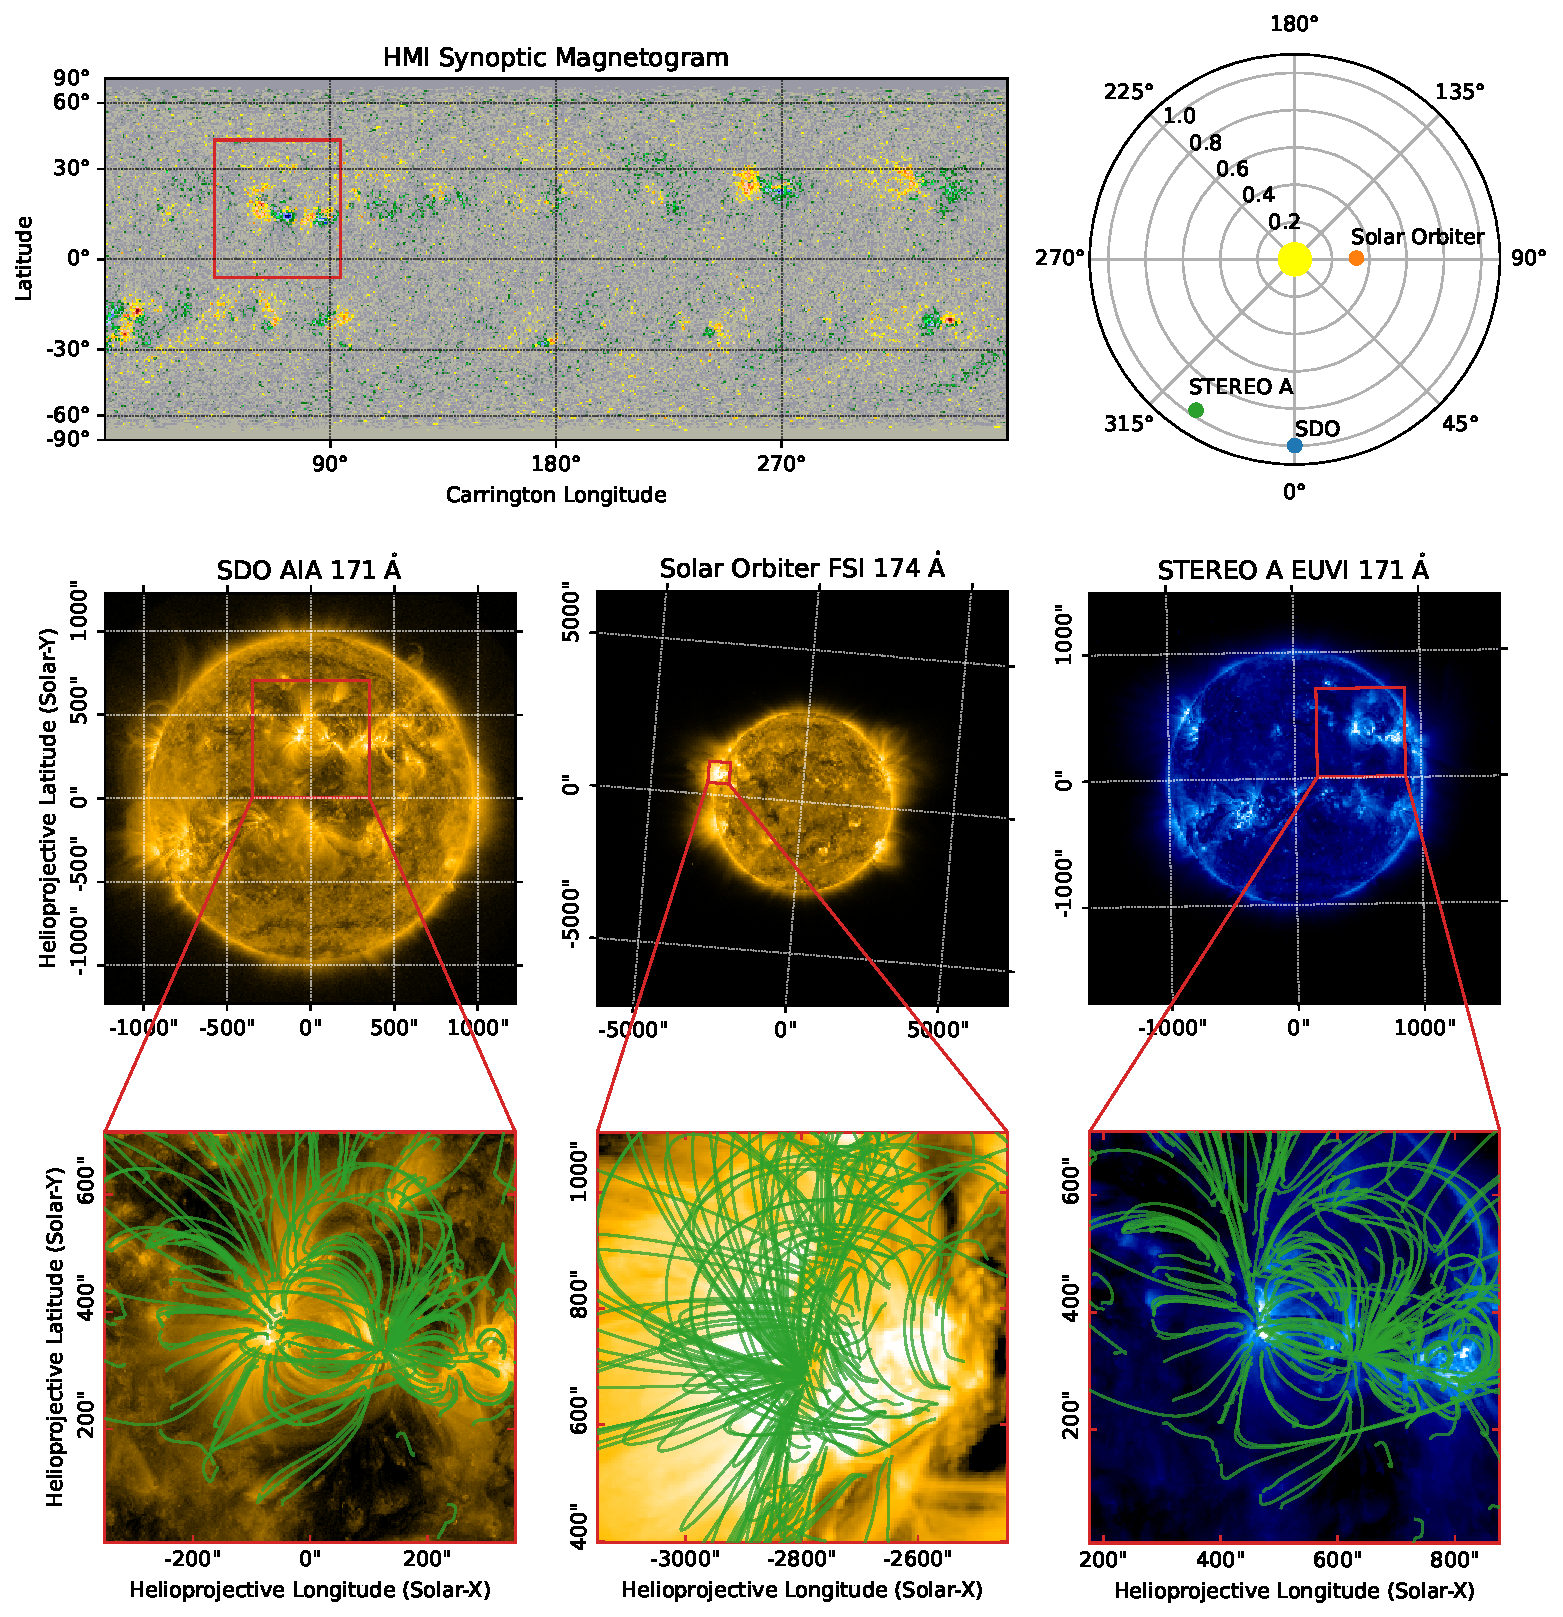
\includegraphics[width=\columnwidth]{figures/loops-multi-viewpoint.pdf}
    \caption{
        Illustration of multiple affiliated packages, including \sunpypkg, \soarpkg, \aiapypkg, and \pfsspypkg, working together.
        \textbf{Top row:} The left panel shows the HMI synoptic magnetogram for Carrington rotation 2255. The red box is centered on the \AR\deleted[id=WTB]{that appeared near disk center on 2022-03-29 21:04 UTC}. The right panel shows the \hgs longitude and radius (in AU) for SDO, STEREO A, and \textit{Solar Orbiter} on 2022-03-29.
        \textbf{Middle row:} Full disk images from SDO AIA at 171 Å (left), SolO FSI at 174 Å (middle), and STEREO-A EUVI at 171 Å (right)\deleted[id=WTB]{ at approximately 2022-03-29 21:00 UTC}. All three images were downloaded using \sunpypkg along with \soarpkg to query the SOAR for the \textit{Solar Orbiter} image. The AIA image was calibrated using \aiapypkg.
        The red box in each panel is centered on the AR shown in the top panel\deleted[id=WTB]{ and has a width and height of 700 arcseconds}.
        \textbf{Bottom row:} Cutouts of the regions denoted in each image in the middle row.
        \added[id=WTB]{\pfsspypkg is used to compute a potential magnetic field solution from the magnetogram (top row) and trace field lines through the resulting volume.
        These field lines are shown in green are transformed to the appropriate coordinate system of each instrument using \sunpypkg}.
    }
    \label{fig:affiliated-package-showcase}
\end{figure}

Since we are interested in the EUV observations of \AR 12976, we also use \Fido to query the VSO for data from AIA on SDO and the Extreme Ultraviolet Imager (EUVI) on the \textit{Solar Terrestrial Relations Observatory} \citep[STEREO,][]{howard_sun_2008}.
Additionally, we use the \package{sunpy-soar} package to allow \Fido to search for and download data from the SOAR.
Here, we query the SOAR for data from the Extreme Ultraviolet Imager \citep[EUI,][]{rochus_solar_2020} on \textit{Solar Orbiter} \citep{muller_solar_2020}.

The middle row of \autoref{fig:affiliated-package-showcase} shows full disk EUV images from AIA (left), the full-sun imager (FSI) on EUI (middle), and EUVI on the STEREO-A spacecraft (right).
We use the \aiapypkg package to correct the AIA image (middle panel) for instrument degradation and update the pointing information.
The red box in each panel is centered on \AR 12976, as seen from the respective spacecraft, and has a width and height of 700 arcseconds.
The top right panel of \autoref{fig:affiliated-package-showcase} shows the \hgs longitude and radius (in AU) of SDO, STEREO-A and \textit{Solar Orbiter} as derived from the observer location metadata of each image.

Viewing the \AR from the vantage points of these three spacecraft (separated by $>90^{\circ}$), we gain a better understanding of its three-dimensional structure.
Additionally, we use the \package{pfsspy} package to compute a potential field extrapolation from the corresponding synoptic magnetogram as shown in the top row of \autoref{fig:affiliated-package-showcase}.
We trace field lines from areas of negative magnetic flux inside the red box corresponding to \AR 12976.
The resulting field lines are overlaid in green on top of the cutouts from each EUV image in the bottom row of \autoref{fig:affiliated-package-showcase}.
Each field line traced using \package{pfsspy} is an \astropypkg coordinate object expressed in terms of a \hgc coordinate frame defined in \sunpypkg.
As such, it is straightforward to transform each field line to the observer-dependent coordinate frame of each image as defined by corresponding observatory using the plotting functionality provided in \astropypkg.
The interoperability between \astropypkg, \sunpypkg, \package{sunpy-soar}, \aiapypkg, and \package{pfsspy} allows us to easily examine the three-dimensional magnetic structure of the \AR and see to what extent the derived potential field corresponds to the EUV emission as observed by these three spacecraft.
